\documentclass[a4paper,12pt]{article}
\title{Inteligencja Obliczeniowa - Projekt 2}
\author{Krzysztof Kołodziejski}
\usepackage{amsfonts}
\usepackage{amsmath}
\usepackage{amssymb}
\usepackage{graphicx}
\usepackage[utf8]{inputenc}
%\usepackage[cp1250]{inputenc}
\usepackage[T1]{fontenc}


\begin{document}
	\maketitle
	\section {Film: The Room}
	\begin{center}
		{
\includegraphics[width=10cm]{johnny.jpg}}\\
	\end{center}
	The Room będący jednym z najgroszych filmów jakie powstały, został napisany przez Tommyego Wisseau który również wyreżyserował owy film i zagrał w nim główną rolę.
	Film składa się z niepowiązanych scen, lecz istnieje w nim zarys fabuły opierający się na trójkącie miłosnym głównego bohatera.
	Mimo tego że The Room jest uważane za jeden z najgorszych filmów, jest zły aż do tego stopnia że staje się śmieszny i zabawny. Właśnie dlatego uznałem że ten film dobrze posłuży do przedstawienia paczek oceniających emocje w tekście.
	\clearpage
	\section {Wykorzystywane paczki oceniające emocje}
	\subsection{Vader}
	Vader ocenia tekst bazując na 3 emocjach. Neutralne, pozytywne, negatywne, niestety paczka większość wypowiedzi traktuje jako neutralne.
	\subsection{Text Blob}
	Text Blob ocenia zdanie w przedziale od -1 do 1, -1 oznacza zdanie maksymalnie negatywne natomiast 1 maksymalnie pozytywne. W ten sposób możemy rozpoznać czy zdanie jest negatywne, neutralne bądź pozytywne.
	\subsection{Text2Emotion}
	Text2Emotion działa już dla 5 emocji dzięki czemu otrzymujemy lepszy obraz osoby przedstawionej w filmie.
	Emocje to: radość, strach, smutek, zaskoczenie i gniew.
	Dzięki tym 5 statystykom łatwo możemy ocenić jaką rolę dana postać odgrywa w filmie, jak i gatunek filmu.
	\subsection{NRCLex}
	NRC Lexicon jest paczką która potrafi rozpoznać aż do 10 emocji, działa bardzo sprawnie ponieważ jedno słowo może zawierać w sobie wiele emocji.
	\clearpage
	\section {Wyniki dla poszczególnych postaci}
	\subsection{Lisa}
	\begin{center}
		{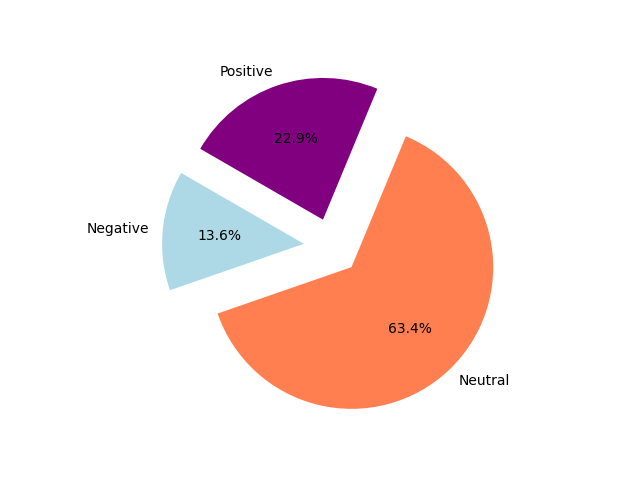
\includegraphics[width=5.5cm]{lisasVaderEmotionalPie.png}}
		{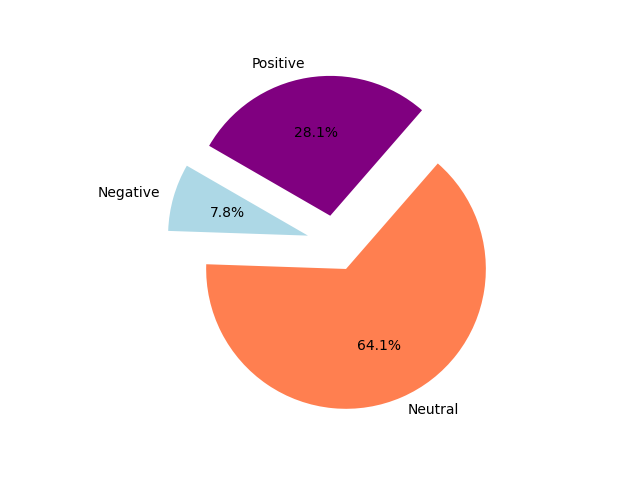
\includegraphics[width=5.5cm]{lisasBlobEmotionalPie.png}}
		{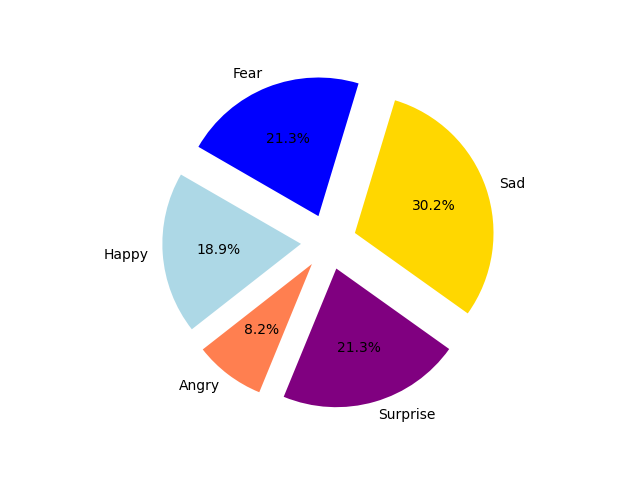
\includegraphics[width=5.5cm]{lisasEmotionalPie.png}}\\
		{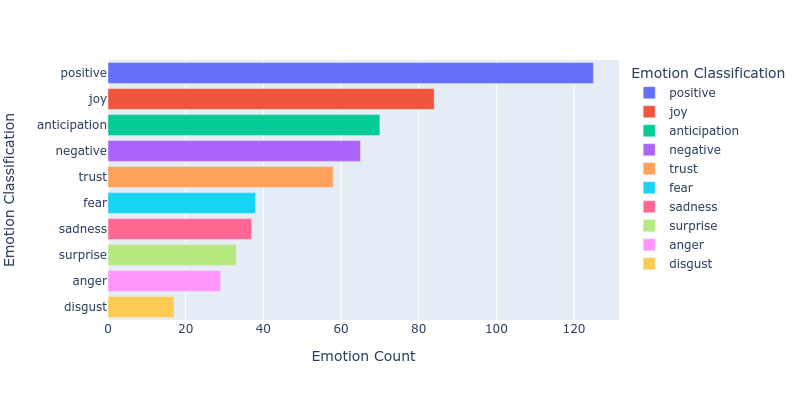
\includegraphics[width=16cm]{lisaNrcImage.png}}\\
	\end{center}
	\clearpage
	\subsection{Johnny}
	\begin{center}
		{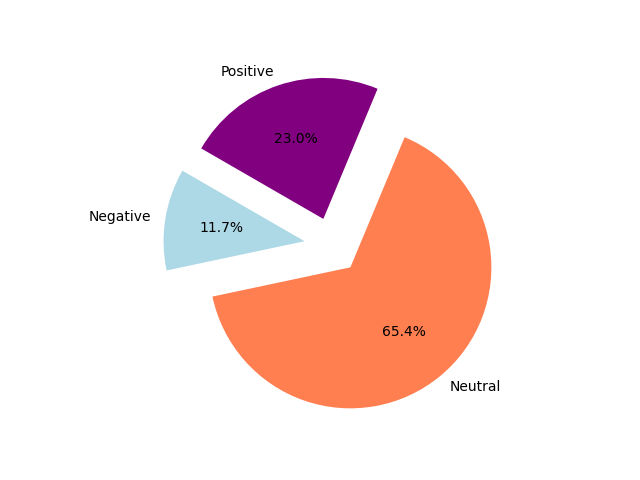
\includegraphics[width=5.5cm]{johnnysVaderEmotionalPie.png}}
		{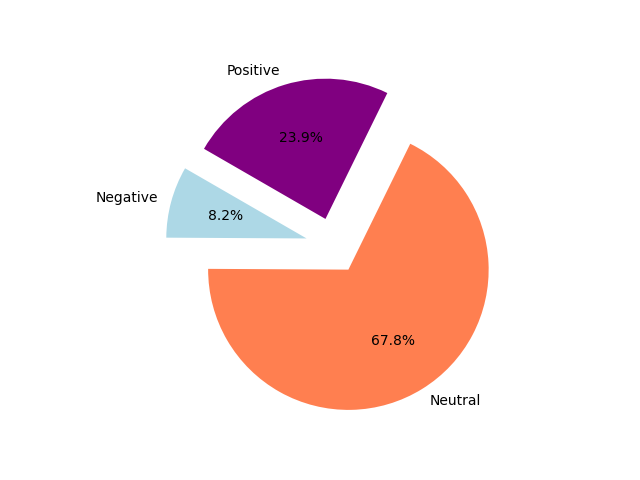
\includegraphics[width=5.5cm]{johnnysBlobEmotionalPie.png}}
		{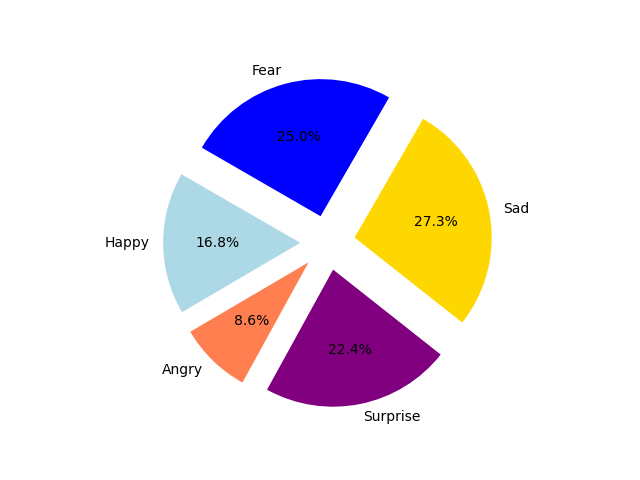
\includegraphics[width=5.5cm]{johnnysEmotionalPie.png}}\\
		{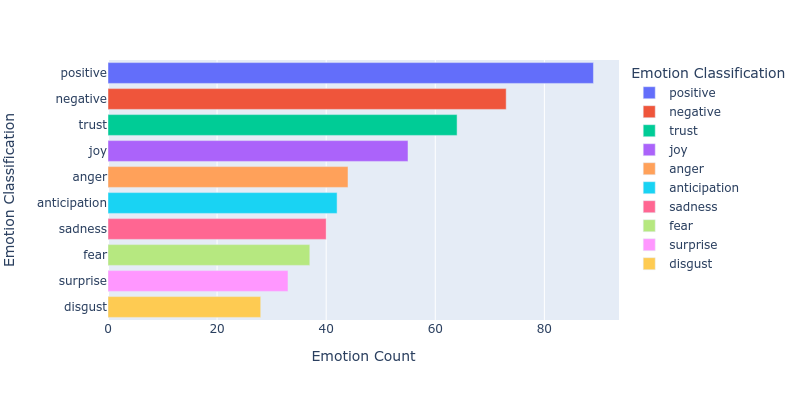
\includegraphics[width=16cm]{johnnyNrcImage.png}}\\
	\end{center}
	\clearpage
	\subsection{Mark}
	\begin{center}
		{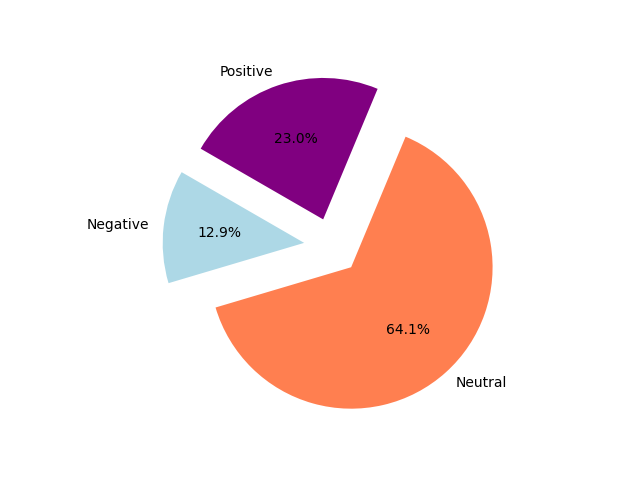
\includegraphics[width=5.5cm]{marksVaderEmotionalPie.png}}
		{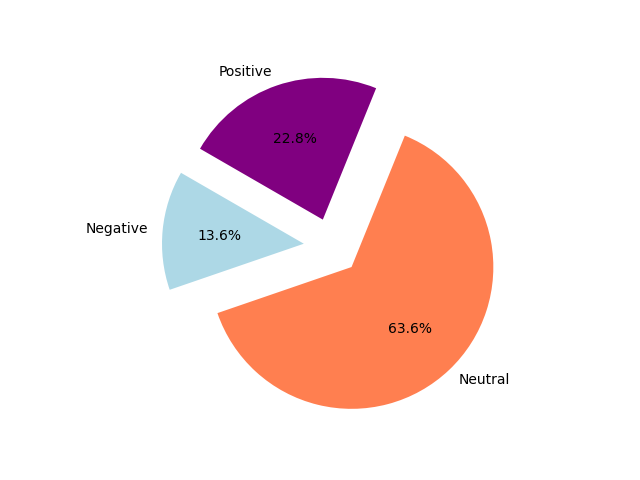
\includegraphics[width=5.5cm]{marksBlobEmotionalPie.png}}
		{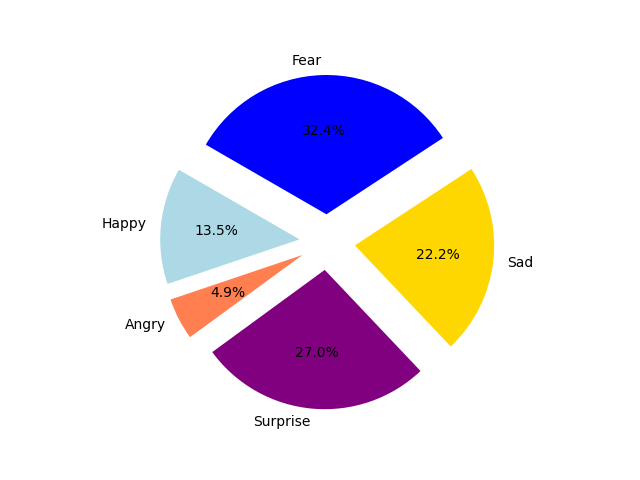
\includegraphics[width=5.5cm]{marksEmotionalPie.png}}\\
		{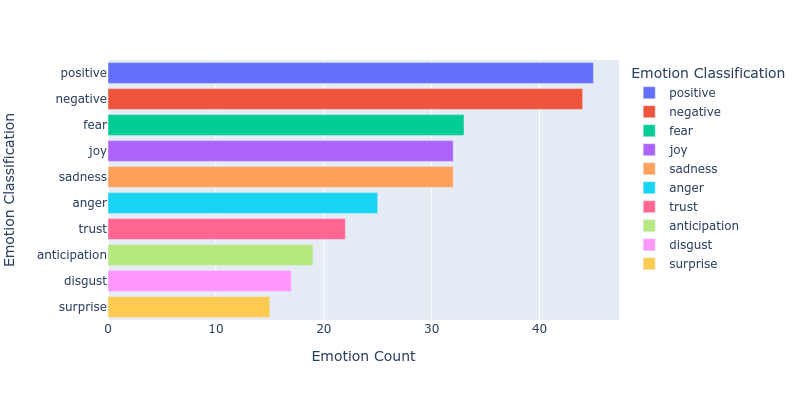
\includegraphics[width=16cm]{markNrcImage.png}}\\
	\end{center}
	\clearpage
	\subsection{Claudette}
	\begin{center}
		{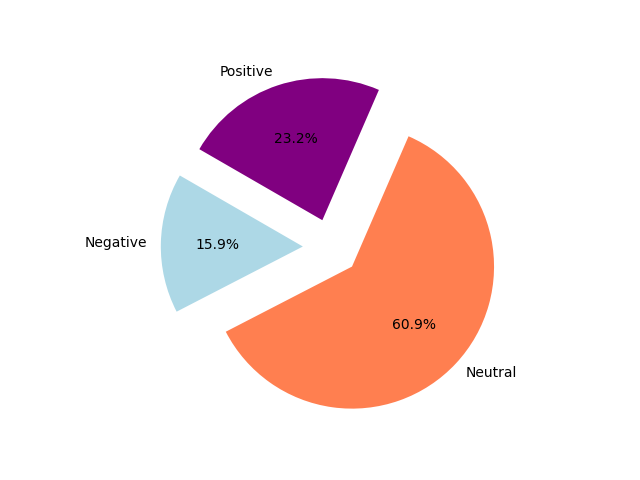
\includegraphics[width=5.5cm]{claudettesVaderEmotionalPie.png}}
		{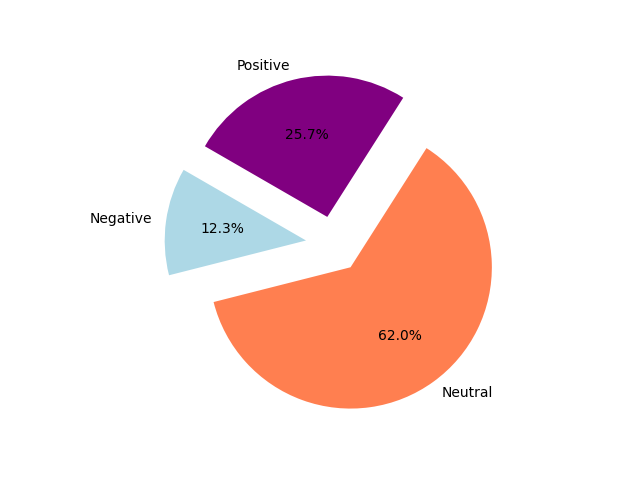
\includegraphics[width=5.5cm]{claudettesBlobEmotionalPie.png}}
		{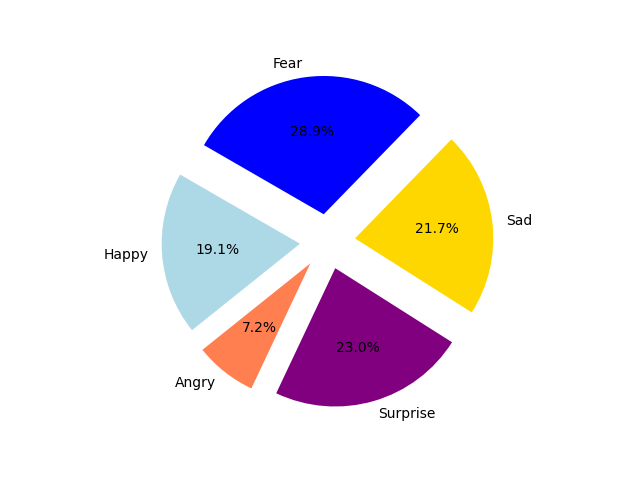
\includegraphics[width=5.5cm]{claudettesEmotionalPie.png}}\\
		{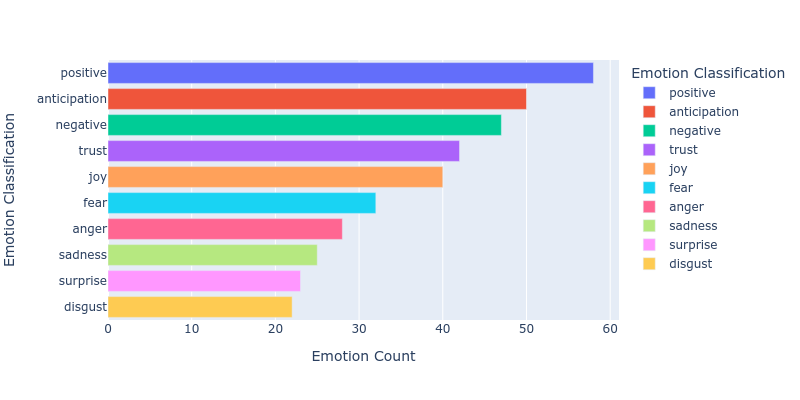
\includegraphics[width=16cm]{claudetteNrcImage.png}}\\
	\end{center}
	\clearpage
	\subsection{Michelle}
	\begin{center}
		{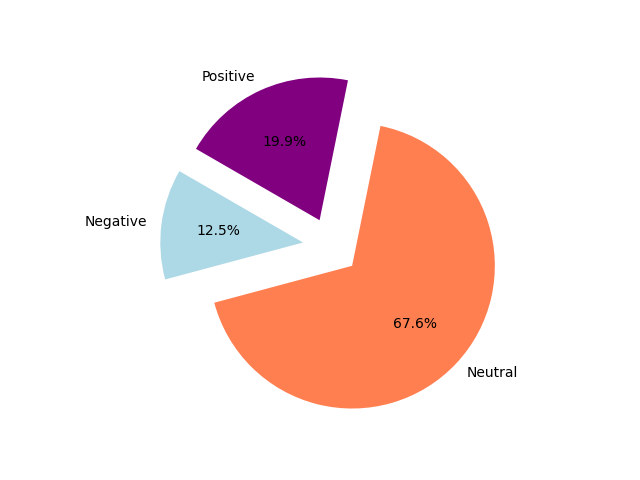
\includegraphics[width=5.5cm]{michellesVaderEmotionalPie.png}}
		{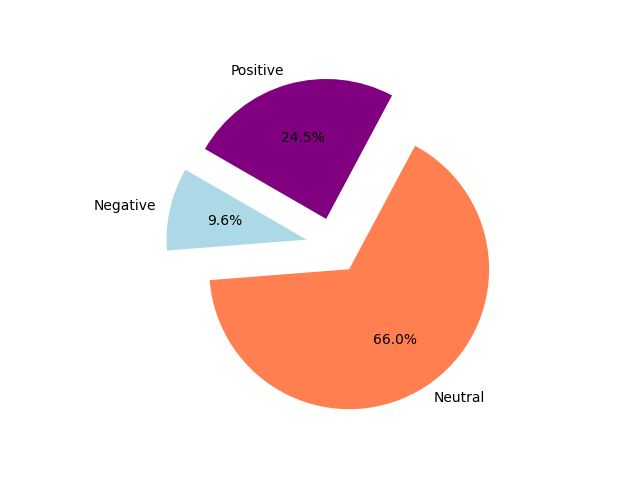
\includegraphics[width=5.5cm]{michellesBlobEmotionalPie.png}}
		{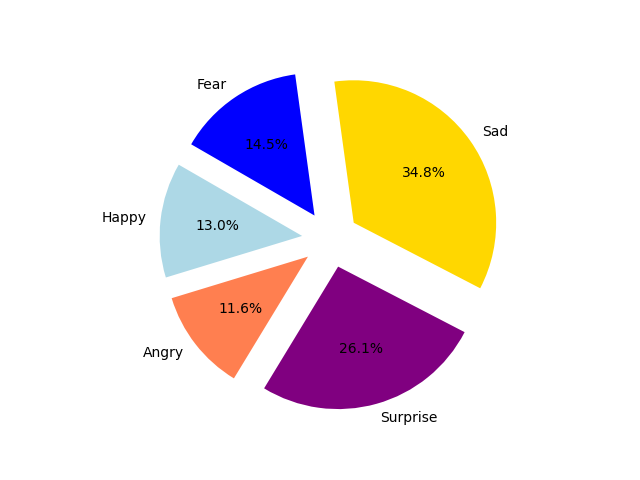
\includegraphics[width=5.5cm]{michellesEmotionalPie.png}}\\
		{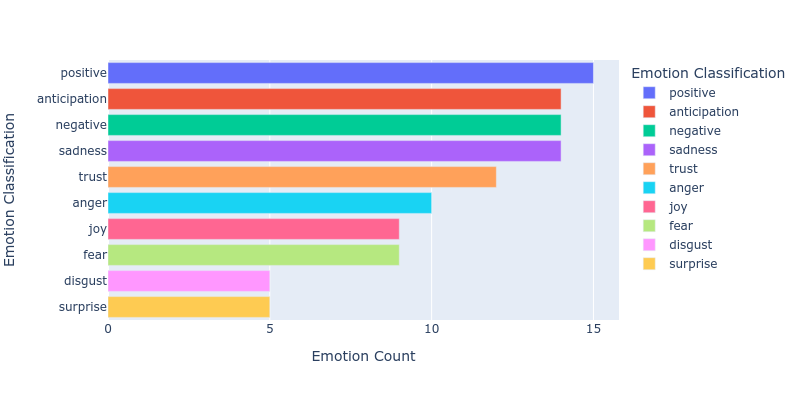
\includegraphics[width=16cm]{michelleNrcImage.png}}\\
	\end{center}
	\clearpage
	\subsection{Peter}
	\begin{center}	
		{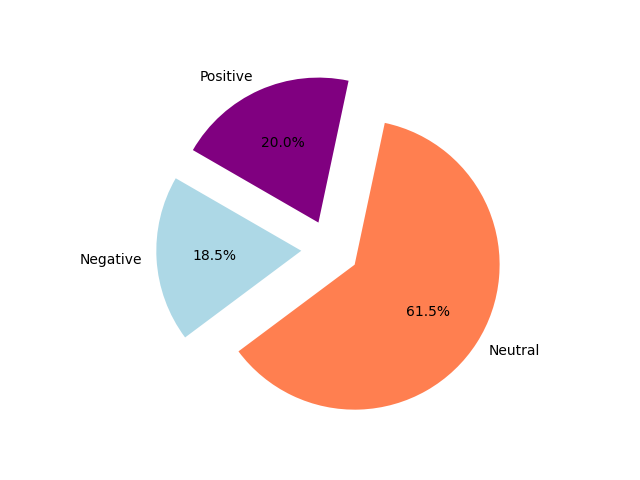
\includegraphics[width=5.5cm]{petersVaderEmotionalPie.png}}
		{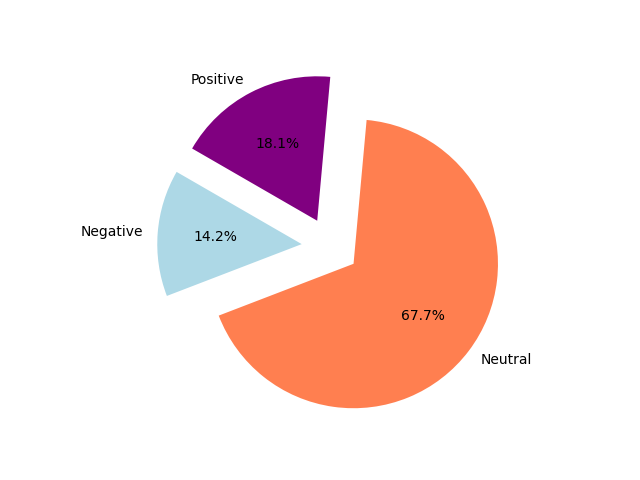
\includegraphics[width=5.5cm]{petersBlobEmotionalPie.png}}
		{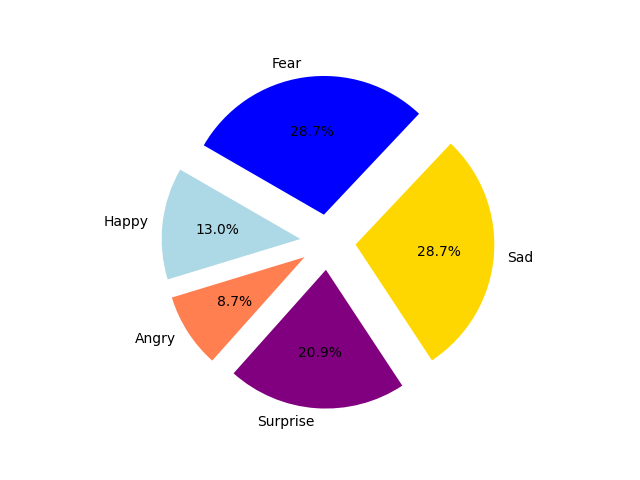
\includegraphics[width=5.5cm]{petersEmotionalPie.png}}\\
		{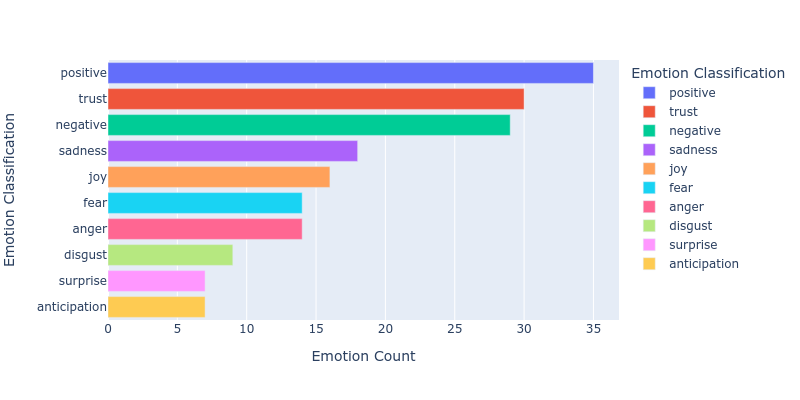
\includegraphics[width=16cm]{peterNrcImage.png}}\\
	\end{center}
	\clearpage
	\section {NRC Lex}
	Pomimo tego iż moim zdaniem Text2Emotion jest bardziej praktyczne do oceniania emocji w tekście, ponieważ ilość informacji jest odpowiednia, to NRC Lex zasługuje na odrobinę uwagi. NRC przypisuje każdemu słowu odpowiadającą mu emocję, ciekawy jest przypadek ze słowem pieniądze które jest wręcz naczyniem wypełnionym pozytywnymi jak i negatywnymi emocjami.\\
	\begin{center}
	{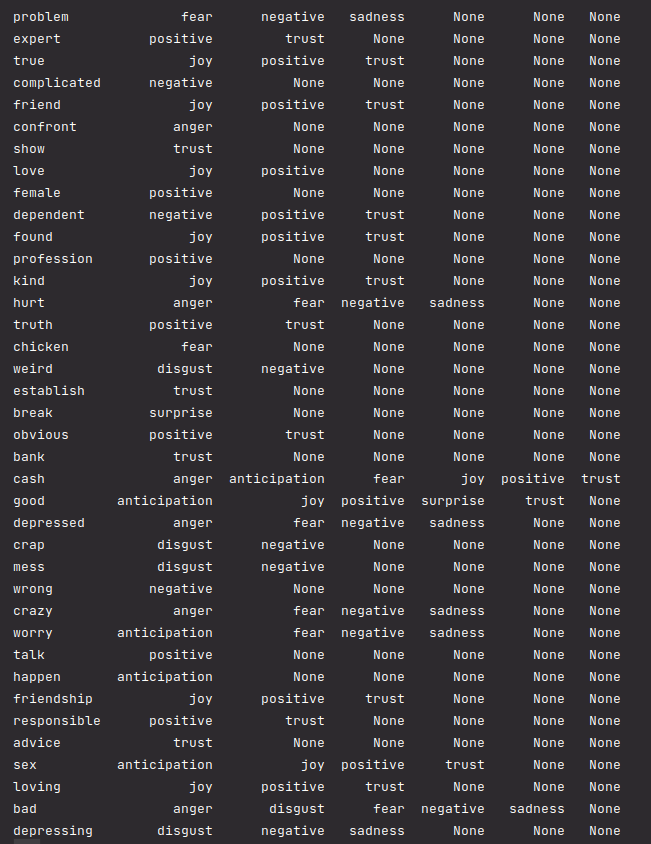
\includegraphics[width=10.5cm]{NRCWords.png}}
	\end{center}
	\clearpage
	\section {Zliczanie słów poszczególnych postaci}
	Analizując słowa wypowiadane przez aktorów, jesteśmy w stanie zobaczyć że Tommy Wisseau nie jest wybitnym scenatzystą ponieważ słowo I dominuje w wypowiedziach.
	Równocześnie po ilości słów widzimy kto odgrywa główną rolę w filmie.
	\subsection{Lisa i Johnny}
	\begin{center}
		{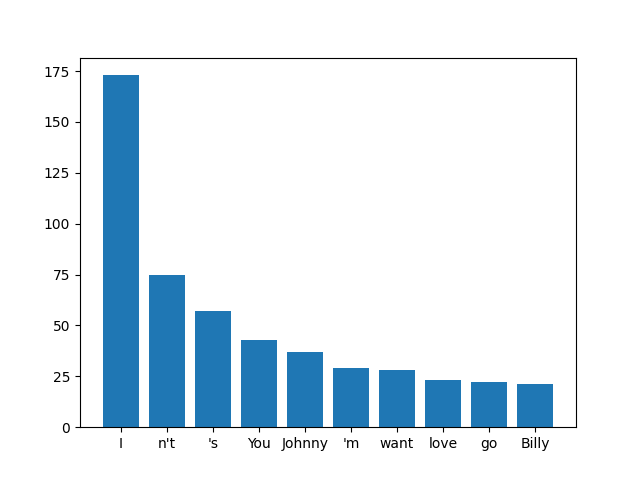
\includegraphics[width=5.5cm]{lisasMostCommonWords.png}}
		{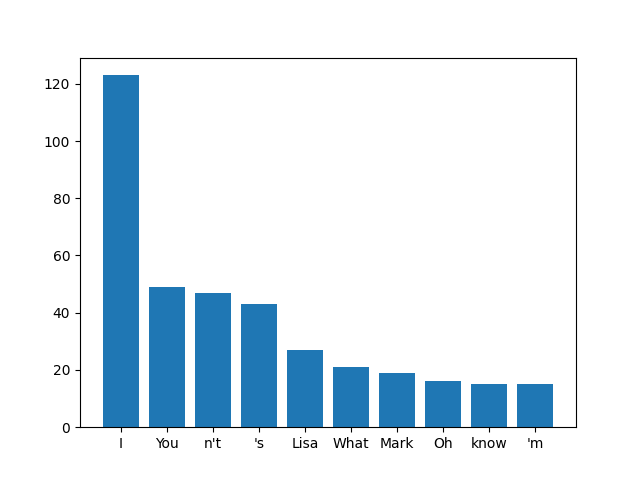
\includegraphics[width=5.5cm]{johnnysMostCommonWords.png}}\\
	\end{center}
	\subsection{Mark i Claudette}
	\begin{center}
		{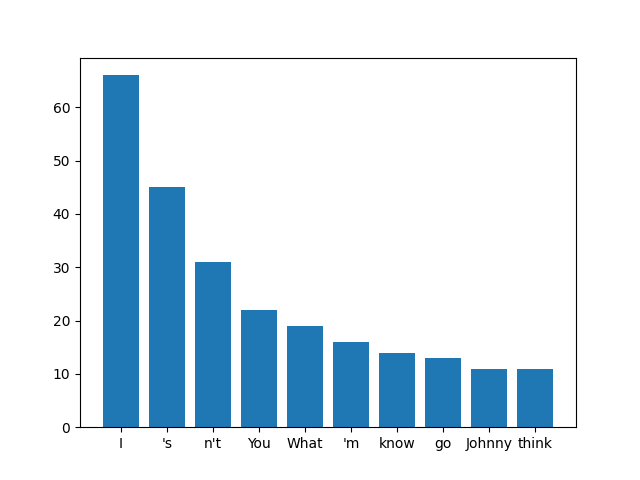
\includegraphics[width=5.5cm]{marksMostCommonWords.png}}
		{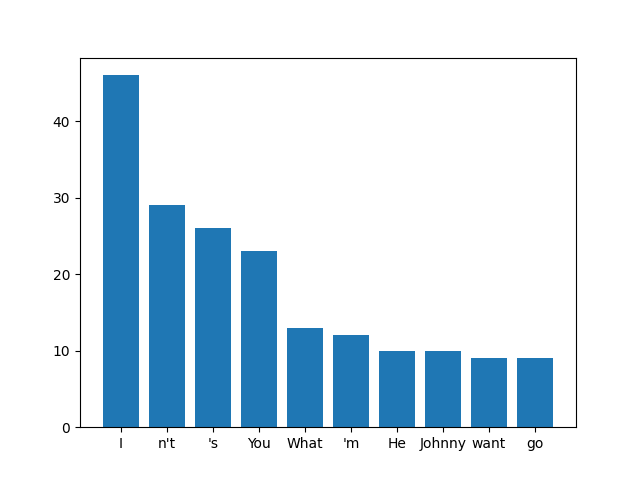
\includegraphics[width=5.5cm]{claudettesMostCommonWords.png}}\\	
	\end{center}
	\subsection{Michelle i Peter}
	\begin{center}
		{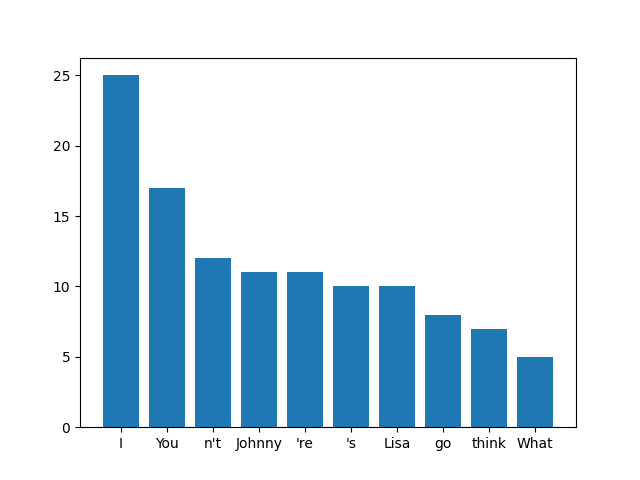
\includegraphics[width=5.5cm]{michellesMostCommonWords.png}}
		{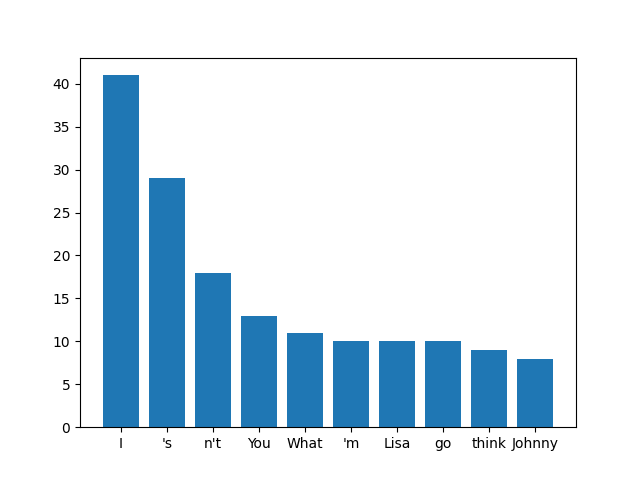
\includegraphics[width=5.5cm]{petersMostCommonWords.png}}\\
	\end{center}
\end{document}